\chapter{Battery SOC Estimation Algorithms}\label{ch:Battery_SOC_Estimation_Algorithms}
We require high-power storage batteries to meet the energy needs of multiple systems. The Lithium-ion batteries are the most popular varieties. Due to their safety, electrochemical structure, high number of charge/discharge cycles, high voltage, and high energy density, they are the most ideal rechargeable battery technologies. This battery type requires a particular charge technique called Constant Current- Constant Voltage (CC-CV) \cite{Coulomb_Counting_SOC_Estimation}.

\section{Coulomb Counting Algorithm (CC)}

State of Charge (SoC) is the most crucial characteristic to keep an eye on to prevent overcharging and deep drain, which can harm the battery's internal structure and even hurt safety.
For estimating the SoC of the lithium-ion battery, several methodologies have been put out in the literature. Both direct and indirect techniques are included in this category. The Coulomb Counting (CC) approach, which takes into account an initial value of SoC (SoC0), and updates it by integrating the current over the nominal capacity, is one example of a direct method that we notice. The CC algorithm has some drawbacks, and the Enhanced CC (ECC) fixes those drawbacks. Using information extracted from the SoC-OCV curve, the open circuit voltage (OCV) estimation is performed.

There are several strategies for indirect methods that can be divided into model-based methods, such as electrical and electrochemical models, and adaptive models, such as the Kalman filter, neural network, or fuzzy logic.
For the model-based ones, certain techniques need for the characterization of the model parameters from a fresh battery, which is expensive and time-consuming. Some of these techniques also can't be used online and call for an understanding of the battery's chemical composition. Due to their great complexity, adaptive models struggle with battery model efficiency and require a significant amount of data training.

The ratio of the nominal capacity to the current capacity is known as the SoC. The CC approach involves taking into account a starting SoC0 value and then updating it by integrating the current over time.
The CC approach has some inefficiencies. In actuality, the SoC0 value is not predetermined, and this method does not take into account the aging factor that influences the Qnom value or the self-discharge phenomenon after extended storage. An ECC approach is suggested as a solution to these problems.
To determine the SoC0 value at each cycle and subsequently update the $100\%$ SoC value, this algorithm takes into account the self-discharging losses and presents a recalibration method for battery propriety at a fully charged state and an empty state.

\begin{equation}\label{eq:batt_SOC_def}
    SOC = \frac{Q_{act}}{Q_{nom}}
\end{equation}

\begin{equation}\label{eq:batt_SOC_CC}
    SOC = SOC_0 + \int_{t_0}^{t_0 + dt} \frac{i_{batt}}{Q_{nom}} 
\end{equation}
\section{Kalman Filter}\label{sec:KalamanFilter}
The Ampere-counting approach is thought to be the most accurate way; nonetheless, it is subject to certain requirements, including a starting SOC value and a regular full charge or full-discharge. 
Due to the measurement error accumulation, it is sometimes impossible to compute SOC directly from current measurements in some applications where these requirements (full-charge or full-discharge) are not always met. For these applications, it is possible to estimate the SOC by using a mathematical model to represent the dynamic properties of the battery and an estimator that monitors battery output measurements and produces an estimation value of the SOC that minimizes the difference between the outputs of the battery and the model.

In chapter \ref{ch:Battery_Modeling_Emulation}, I have extensively discussed the battery One-Time and Two-Time constant equivalent models. I have also attempted to describe the mathematical model of the battery in section \ref{sec:Batt_Modeling} and chapter \ref{ch:Battery_Modeling_Emulation} as the rock-solid fundamental basis for the Kalman filter.
The battery parameters used in the Kalman filter($R_0,R_{OTC}, C_{OTC}, V_{OTC}$) to calculate the SoC extracted from the voltage SOC graphs (elaborated in section \ref{sec:Batt_model_parameters_estimation} ) of the battery. In this section, I have attempted to implement the One-Time constant model of the battery through the Kalman filter. All the modeling equations(eq.\ref{eq:OTC_Voltage }, \ref{eq:Discrete_OTC_Voltage } and 4.3 ) used in the Kalman algorithm are taken from the battery OTC equivalent circuit(Figure \ref{fig:Battery_Equivalent_circuit}(b)).

In essence, a Kalman filter is a system of recursive equations that implements a predictor-corrector type estimator. It creates an ideal guess of the system state based on the input control and output measurements; as a result, it is typically employed when the system state cannot be directly monitored and needs to be predicted optimally from the output measurements \cite{SOC_Estimation_KalmanFilter_Ahmad}.
In this section \ref{sec:KalamanFilter}, the extended Kalman filter (EKF) for non-linear systems is explained, followed by the discrete Kalman filter for linear systems, and lastly a state space model for the Li-Ion battery is built up. To assess the reliability of the suggested method, comparisons are also made between SOC values calculated by Ampere-counting and SOC values estimated by EKF \cite{SOC_Estimation_KalmanFilter_Liu}.

\subsection{The Discrete Kalam Filter}\label{sec:Discrete_Kalam_Filter}
This section outlines the fundamental design of a Kalman filter, which takes measurements and estimates the system state at discrete time intervals \cite{LIPO_Batt_Parameters_identification_Rahmoun}.

The linear difference stochastic equation \ref{eq:Discrete_State_Equation} governs a discrete time-controlled process, and the problem of estimating the state vector $x_k \in \mathfrak{R}^m$ of this process is handled by the discrete Kalman filter.

\begin{equation}\label{eq:Discrete_State_Equation}
    x_{k+1} = A_k x_k + B_k u_k + w_k
\end{equation}
where the measurement vector $y_k \in \mathfrak{R}^m $ is given by \ref{eq:Discrete_Measurement_Output_Equation}.
\begin{equation}\label{eq:Discrete_Measurement_Output_Equation}
    y_{k} = C_k x_k + D_k u_k + v_k
\end{equation}

Equation \ref{eq:Discrete_State_Equation} is referred to as a "state equation" or "process equation".This equation explains the dynamics, stability, controllability, and disturbance sensitivity of the system.
The control input to the system is $u_k \in \mathfrak{R}^p$, and $w_k \in \mathfrak{R}^n$ is a random variable that represents the "process noise" \cite{SOC_Estimation_KalmanFilter_Ahmad}.
The output equation of the discrete system is represented in the equation \ref{eq:Discrete_Measurement_Output_Equation}, the output state equation defines the dependency on the state vector $x_k$, control input $u_k$ and $v_k \in \mathfrak{R}^{m}$, Which models the measurement noise in the system.

The matrix $A_k \in \mathfrak{R}^{n\times n}$ describes the system dynamics and
relates the state at the previous time step $k-1$ to the state at
the current time step k when the control input $u_k$ is zero. The
matrix $B_k \in \mathfrak{R}^{n\times p}$ relates the control input $u_k$ to the state $x_k$.
The matrices $C_k \in \mathfrak{R}^{m\times n}$ and $D_k \in\mathfrak{R}^{m\times p}$ relate the measurement
$y_k$ to the state $x_k$ and control input $u_k$. All these matrices can be time-varying which can be extensively described through the Extended Kalman Filter.

Given a system model, a known control input $u_k$, a known measurement $y_k$, and certain assumptions, the Kalman filter approach can provide the most accurate estimation of the unmeasured state value $x_k$.
First, it is assumed that both wk and $v_k$ are mutually uncorrelated white Gaussian random processes with zero mean and known values for the covariance matrices.

\begin{equation}\label{eq:Discrete_Noise_Covariance}
    P(w) \sim N(0,Q) ; \\
    P(v) \sim N(0,R) \\
\end{equation}
Process noise covariance Q and measurement noise covariance R might change with each time step, but here we assume that they are constants  \cite{SOC_Estimation_KalmanFilter_Ahmad}.
The system must also be "observable," which means that it must be feasible to infer its state from its output. This criterion is met by the system we are developing.

\begin{figure}
        \centering
        \begin{tikzpicture}[node distance=2cm]
            \node (start) [startstop] {
                \makecell[l]{Initial Estimate $x_{0/0}$ and \\ 
                            Error Covariance $P_0$, Q, and R}
            };
            \node (in1) [io, below of=start,yshift=-1cm] {
                \makecell {
                    \textbf{State Prediction} \\
                    Determine State\\
                    $\hat{x_{k + 1/k}} = A \hat{x_{k/k}}  + B u_k$\\
                    Determine output\\
                    $\hat{y_{k + 1}} = C \hat{x_{k/k}} + D u_k$\\
                }
            };
            \node (pro1) [process1, below of=in1,yshift=-2.25cm] {
                \makecell{ 
                    \textbf{Error Covariance} \\
                    $P_{k + 1/k} = A P_{k/k} A^T + R$\\
                }
            };
            \node (pro2) [process2, right of=pro1, xshift=5cm] {
                \makecell{ 
                    \textbf{ Correction} \\
                   Determine Kalman Gain\\
                   $K_{k + 1} = P_{k + 1/k} C^T [C P_{k + 1/k} C^T + Q]^{–1}$\\
                   Employ Correction on Prediction of States\\
                   $\hat{x_{k + 1/k + 1}} = \hat{x_{k + 1/k}} + K_{k + 1} [y_{k + 1} –  \hat{y_{k + 1}}]$ \\
                   Determine Error Covariance\\
                   $P_{k + 1/k + 1} = [I – K_{k + 1} C] P_{k + 1/k}$\\
                }
            };
            \draw [arrow] (start) -- (in1);
            \draw [arrow] (in1) -- (pro1);
            \draw [arrow] (pro2) |- (in1);
            \draw [arrow] (pro1) -- (pro2);
        \end{tikzpicture}
        \caption{Discrete Kalman Filter Algorithm Flow Chart}
        \label{algo:Discrete_Kalman_Filter_Algorithm_Flow_Chart}
\end{figure}


\begin{itemize}
    \item \textbf{Initialization :} Then the state vector $x_0$ and its associated covariance vector $P_0$ for $K=0$ are initialized. Both perturbations, w and v are uncorrelated white Gaussian random processes with known value covariance matrices Q and R are initialized at this step of the algorithm.
    \item \textbf{Prediction :} For each iteration k newly acquired input data, u is injected into the system, Based on the calculated prior state $\hat{x_{k+1/k}}$, the state vector is predicted along with predicted covariance $P_{k+1/k}$.
\end{itemize}

\begin{equation}\label{eq:Discrete_Prior_State_Equation}
    x_{k+1/k} = A_k x_k + B_k u_k 
\end{equation}
\begin{equation}\label{eq:Discrete_Prior_Covariance_Equation}
    P_{k+1/k} = A_k P_k A_k^{T} + Q
\end{equation}

If the system is stable then $A_k P_k A_k^{T}$ is diminished and reduces the uncertainty of the state estimation over time. The process noise term Q always increases the
uncertainty because $w_k$ cannot be measured. The second estimated $\hat{x_{k + 1/k + 1}}$ tunes up the first estimated $\hat{x_{k + 1/k}}$ (prior state) after measuring the system output $y_k$. The state and error covariance $\hat{x_{k + 1/k + 1}}$ and $P_{k + 1/k + 1}$
are more accurate than $\hat{x_{k + 1/k}}$ and $P_{k+1/k}$ as they involve the information from the measurement $y_k$.

The projected state estimation plus a weighted correction factor  $\hat{x_{k + 1/k + 1}} = \hat{x_{k + 1/k}} + K_{k + 1} [y_{k + 1} –  \hat{y_{k + 1}}]$, as illustrated in, equals the updated state estimation, which is denoted by the symbol $K_k$(Kalman gain).
$P_{k+1/k}$ tends to be "big," which results in a large Kalman gain, which results in a large update for the state estimation $\hat{x_{k + 1/k + 1}}$ if the current state estimation $\hat{x_{k + 1/k}}$is highly uncertain.
The current state estimation will only need to be slightly updated if the current state estimation is confident. Additionally, if the measurement noise is strong due to a high R value, this will result in a low Kalman gain and a little update. The signal to noise ratio (SNR) of the sensor is additionally balanced by the Kalman gain. When the sensor's SNR is high, the Kalman gain is low and the filter converges more quickly.
\begin{itemize}
    \item \textbf{Corretion and Update :} A correction factor ($y_{k + 1} –  \hat{y_{k + 1}}$) equal to the system output $ \hat{y_{k + 1}}$ is added to the new measurement $y_k$ to provide fresh information.
\end{itemize}

The best information on the state and error covariance is used to initialize the Kalman filter, as shown in eq . \ref{eq:Kalam_state_and_covaraince_initialize}.
\begin{equation}\label{eq:Kalam_state_and_covaraince_initialize}
    \hat{x_{k/k}} = E[x_{k/k}], P = E[(x_{k/k} - \hat{x_{k/k}})(x_{k/k} - \hat{x_{k/k}})^T]
\end{equation}
Even though it happens frequently that these quantities are not precisely known, the Kalman filter is well renowned for being extremely resilient to improper initialization and will swiftly converge to the correct values as it runs.


\subsection{Extended Kalman Filter}

The extended Kalman filter is the Kalman filter for nonlinear systems. With the extended Kalman filter technique, a linearization procedure is carried out at each time step to approximate the nonlinear system with a linear time-varying system. The extended Kalman filter for the real nonlinear system is produced by using the linear time-changing system in a Kalman filter. Similar to a Kalman filter, an extended Kalman filter assumes that the process noise and sensor noise are independent, zero-mean Gaussian noises and uses the measured input and output to get the minimum mean squared error estimate of the true state \cite{ADIJ_MARTIN2017}.

In the battery pack system equation\ref{eq:Discrete_OTC_Voltage } and 4.3, the system state variables are defined as $x_1(t) = SOC_0$ and $x_2(t) = V_{OTC}$. The input is defined as u(t) = $i_{batt}$ and the output is y(t) = $V_batt$. 
\begin{equation}
    \dot{x}  = f(x,u) + w
\end{equation}
\begin{equation}
    y  = g(x,u) + v
\end{equation}
where $x = [x_1,x_2]^T$, The functions $f(x,u)$  and $g(x,u)$ are :
\begin{equation}\label{eq:Batt_Kalman_State_function}
    f(x,u) =  \begin{bmatrix}
                    \frac{u}{k C_{OTC}} \\
                    -\frac{1}{R_{OTC} C_{OTC}} x_2 + \frac{1}{C_{OTc}} u
               \end{bmatrix}  
\end{equation}
\begin{equation}\label{eq:Batt_Kalaman_output_function}
    g(x,u) = k x_1 + x_2  + R_0 u + d
\end{equation}
the relationship between battery OCV and SOC is only piecewise 
linear in practice, $V_{OC}$(Open circuit voltage ckt. \ref{fig:Battery_Equivalent_circuit}(b)) can be expressed as 
$V_{OC} = K S_{OC} + d$
$V_{OC}$ could also be a polynomial interpolation of the soc.\\

Recalling the battery terminal voltage from model \ref{fig:Battery_Equivalent_circuit}(b):
\begin{equation}\label{eq:Batt_Kalaman_Terminal_Voltage}
    V_{batt} = K S_{oc} + V_{OTC} - I_{batt} R_0 + d
\end{equation}

If the functions f(x,u) and g(x,u) are linearized by a first-order, Taylor 
series expansion, at each sample step about the current operating point, 
the linearized model is 
\begin{equation}\label{eq:Batt_Kalman_State_function_tylor_expansion}
    \delta \dot{x} = A_k \delta x + B_k \delta u
\end{equation}
\begin{equation}\label{eq:Batt_Kalaman_output_function_tylor_expansion}
    \delta y = C_k \delta x + D_k \delta u
\end{equation}

where ;
\begin{equation}\label{eq:Batt_Kalman_function_tylor_expansion_Ak}
    A_k = \frac{d f(x,u)}{d x} =  \begin{bmatrix}
                                        0 & 0 \\
                                        0 & -\frac{1}{R_{OTC} C_{OTC}} 
                                  \end{bmatrix}                          
\end{equation}
\begin{equation}\label{eq:Batt_Kalman_function_tylor_expansion_Bk}
    B_k = \frac{d f(x,u)}{d x} =  \begin{bmatrix}
                                        -\frac{1}{K Q_{tot}} \\
                                         -\frac{1}{ C_{OTC}} 
                                  \end{bmatrix}                          
\end{equation}
\begin{equation}\label{eq:Batt_Kalman_function_tylor_expansion_Ck}
    C_k = \frac{d f(x,u)}{d x} =  \begin{bmatrix}
                                    K & 1\\  
                                  \end{bmatrix}                          
\end{equation}
\begin{equation}\label{eq:Batt_Kalman_function_tylor_expansion_Dk}
    D_k = \frac{d f(x,u)}{d x} =  [R_0]                         
\end{equation}

The battery model represented by equation \ref{eq:Batt_Kalman_State_function_tylor_expansion} and \ref{eq:Batt_Kalman_function_tylor_expansion_Bk} can be discretized as
\begin{equation}\label{eq:Batt_Kalman_State_Prediction}
    x_{k+1} = A_d x_k + B_d u_k 
\end{equation}
\begin{equation}\label{eq:Batt_Kalman_Output_Prediction}
    y_{k+1} = C_d x_k + D_d u_k
\end{equation}

where $A_d \simeq  E + T_c A_k, B_d \simeq  T_c B_k$, E is the unit matrix and $T_c$ is the sampling 
period, and $C_d \simeq  C_k, D_d \simeq  D_k$ . 
\begin{figure}
    \centering
    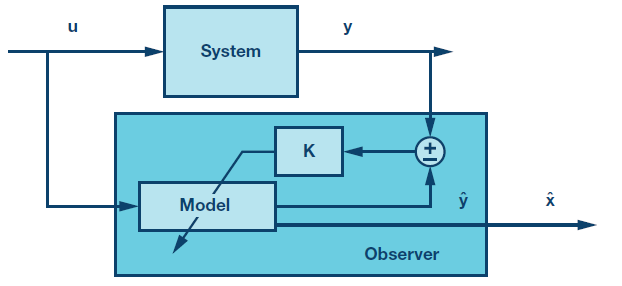
\includegraphics[width=0.5\textwidth]{Chap07/Figures/Kalman_principle.PNG}
    \caption{Kalman Filter Principle}
    \label{fig:Kalman_Filter_Principle}
\end{figure}
The Kalman filter is an ideal observer, and Figure \ref{fig:Kalman_Filter_Principle} shows how it works. The idea is to employ a feedback system that modifies the model's uncertain variables to reduce errors between estimated and measured outputs as they occur in real-time. By using a model fit like this, it is feasible to observe the model's physical parameters that are not measurable. The correction allows for the dynamic and functional correction of the filter and is weighted by a gain vector K. Every iteration uses error forecasts and uncertainties (noise) on states and observations to calculate the gain.
The flowchart \ref {algo:Discrete_Kalman_Filter_Algorithm_Flow_Chart} describes the implementation of the extended Kalman filter and I have also grabbed an opportunity to implement the algorithm through the script (described \ref{sec:Extended Kaman Filter Implementation}). 

\section{Extended Kalman Filter Results Discussion}

\subsection{Charging Mode of the LIPO Batteries :}
The Kalman filter experimentation for estimating the soc was carried out on the 10Ah LiPo battery. Figure general charging profile of the LiPo battery, most appropriate charging procedure is to charge the battery in constant current mode as battery voltage reaches close to 4.2Volts change the batteries in the constant voltage (CV) and let the current drop slowly. This charging profile is demonstrated in Figure 2 to estimate the battery soc from the Kalman filter and amper second method. As a result, 1 LIPO battery has reached charged with 4.1Volt with a constant current of 4.5A somewhere around 30 to 40mins, but the soc of the battery is still at $75\%$ to let the battery charge to $100\%$ SOC the charging mode has been a change from CC to CV and the current slowly dropped to zero.
\begin{figure}[h]
	\centering
	\subfigure[Battery Charging Voltages]{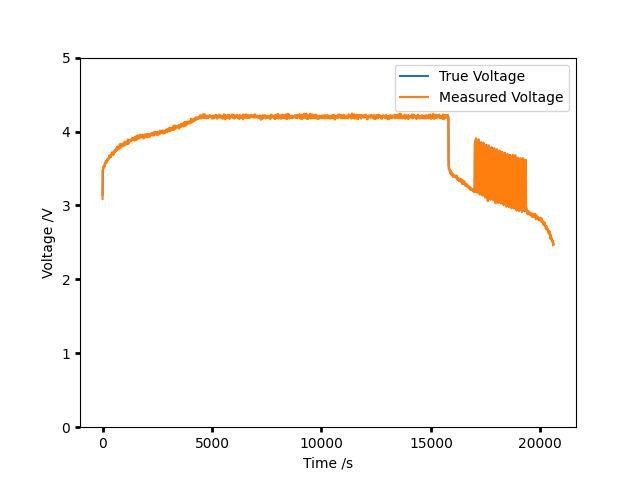
\includegraphics[scale=.4]{Chap07/pyKalmanFilter/Python/Figures/BatteryChargingVoltage.png}}
	\qquad
	\subfigure[Battery Charging Current]{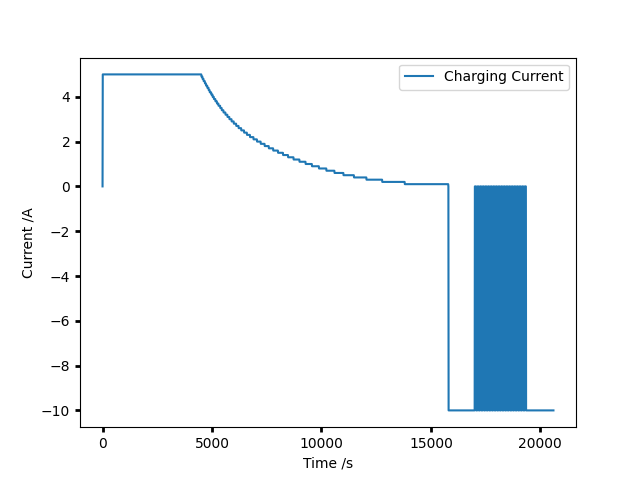
\includegraphics[scale=.4]{Chap07/pyKalmanFilter/Python/Figures/BatteryChargingCurrent.png}}
	\qquad
	\subfigure[Battery Charging SOC]{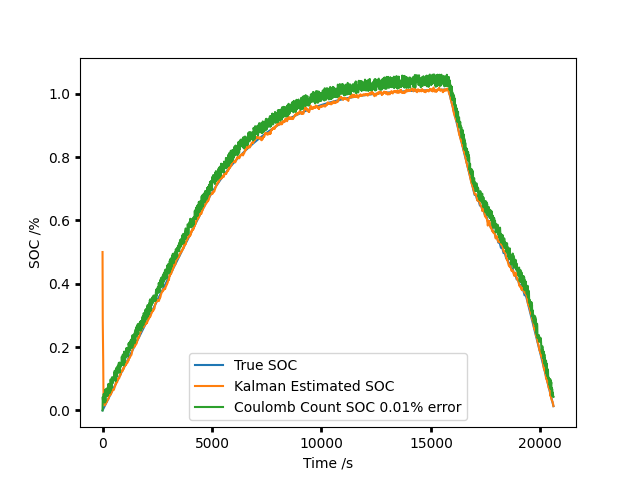
\includegraphics[scale=.4]{Chap07/pyKalmanFilter/Python/Figures/BatteryChargingSOC.png}}
	\qquad
	\subfigure[Battery Charging SOC Error]{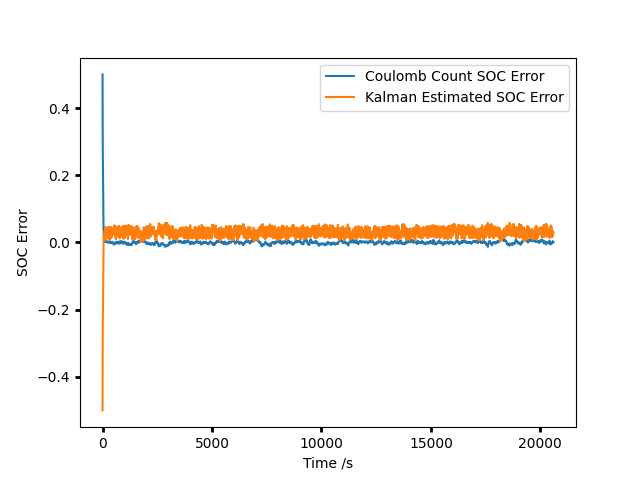
\includegraphics[scale=.4]{Chap07/pyKalmanFilter/Python/Figures/BatteryChargingSOCError.png}}
	\caption{Charging Battery Kalman Filter Results}
	\label{fig:Charging_Battery_Kalman_Filter_Results}
\end{figure}

\subsection{Sampling Time $dt$ :}
In an ideological world, we need to sample the current flowing in the battery to calculate the most accurate soc of the battery, but this is quite difficult to do in the practical world, so we need to discretize the time and take the current sample in $T_c$  or $dt$ time.  As we push the sample time smaller and smaller we are close to estimating the actual current flowing in the battery and soc. On the contrary, if we push measurement time to a very very narrow value there is a high chance that to acquire more measurement noise, and we may end up with wrong estimations. This problem is even more emphasized in the column count method,  well than what is the right sample time; it is very hard to say. It depends on the measurement setup and the charging current profile. I have made a few experiments to demonstrate noise encountering the measuring setup and wrong estimations. 

\begin{figure}
    \centering
    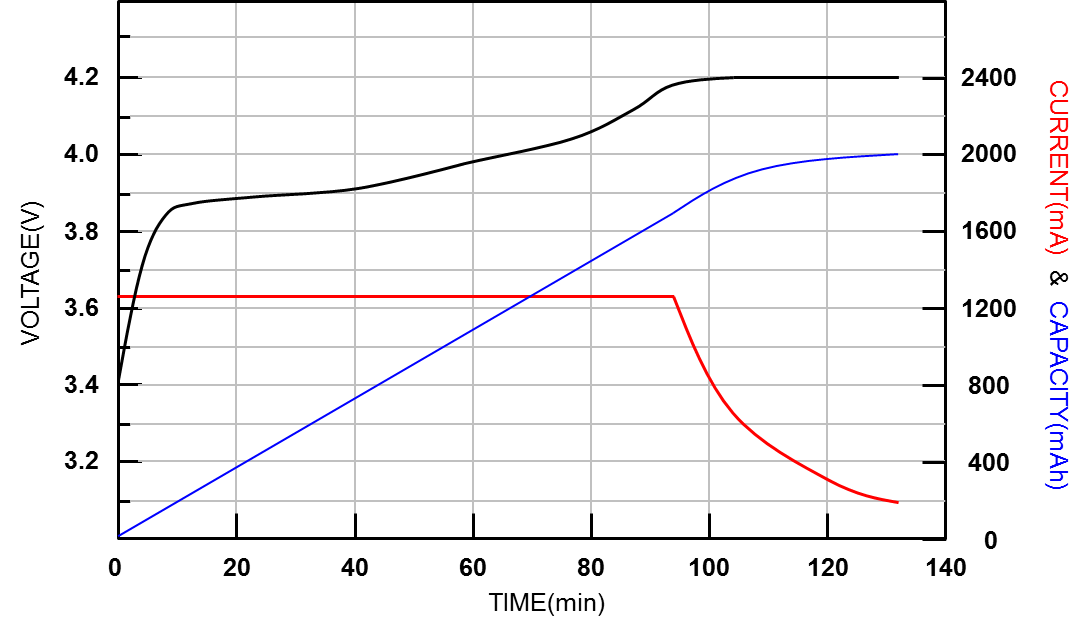
\includegraphics[width=0.5\textwidth]{Chap07/pyKalmanFilter/Python/Figures/Charging-curve-for-Lithium-polymer-battery.png}
	\caption{Charging Profile of the LIPO Batteries}
	\label{fig:Charging_Profile_of_the _LIPO_Batteries}
\end{figure}

\subsection{SOC estimation by Kalman Filter:}
SOC estimated by the Kalman filter is quite satisfactory for this LIPO battery the results have been demonstrated \ref{fig:Charging_Battery_Kalman_Filter_Results}(c) and (d). Figure \ref{fig:Charging_Battery_Kalman_Filter_Results}(c) points out the true soc(SOC profile given by the manufacturer), the Coulomb count method, and Kalman filter soc estimation. The green graph is the Coulomb count soc which is acquired with $0.01\%$ of the random noise in the setup, the results have been quite clear that the Coulomb count method keeps on accumulating the noise and diverging from true soc.
On the contrary Kalman filter encounter a lot of noise at the initial stage because the covariance matrix$P_k$ that we initialized might have far diverged from the measuring values in the system (eq . \ref{eq:Discrete_Noise_Covariance}). As time progresses the algorithm will try to correct the error between the true measurement $y_k$ and the estimated value $\hat{y_k}$ and tune its Kalman gain and approaches to the true soc of the battery.

\begin{figure}[h]
	\centering
	\subfigure[Battery Charging SOC @ $dt$=1mS]{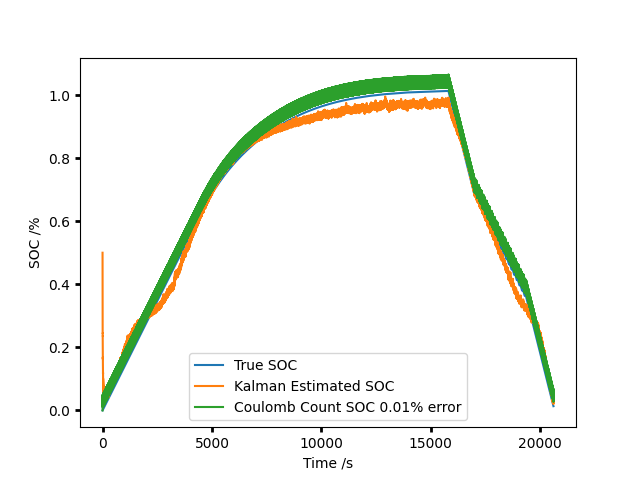
\includegraphics[scale=.4]{Chap07/pyKalmanFilter/Python/Figures/BatteryChargingSOC_dt0_01.png}}
	\qquad
	\subfigure[Battery Charging SOC @ $dt$=1mS]{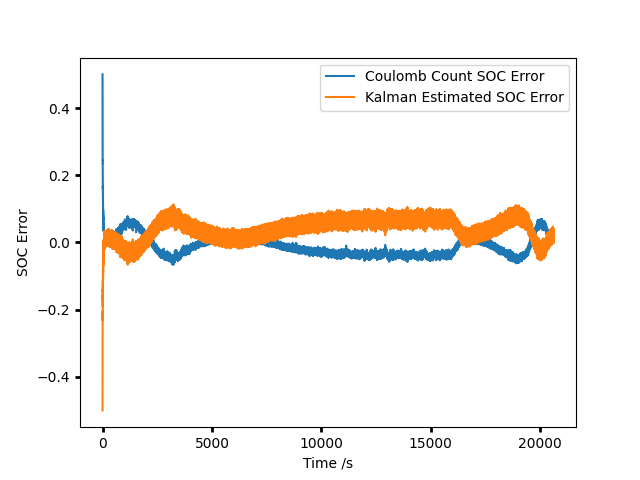
\includegraphics[scale=.4]{Chap07/pyKalmanFilter/Python/Figures/BatteryChargingSOCError_dt0_01.png}}
	\caption{Charging Battery Kalman Filter Results Smaplingtime $dt$ = 1mS}
	\label{fig:Charging_Battery_Kalman_Filter_Results_SamplingTime_1mS}
\end{figure}

Figure \ref{fig:Charging_Battery_Kalman_Filter_Results_SamplingTime_1mS} shows the Kalman and coulomb count soc estimation with a sampling time of 1ms and the error between the true soc to the estimated soc is a lot, even the Kalman filter is oscillating too much to tune the Kalman gain. The Results expressed in figure \ref{fig:Charging_Battery_Kalman_Filter_Results}(c) and (d) are sampled at 100ms with $0.01\%$ measurement noise, the soc estimation is pretty much descent compared to the 1ms results.
The conclusion from this experiment is the sample time Tc is very very important for the SOC estimation even both for the Kalman filter and Ampers second count, but it is not a predefined value it depends on the measurement and data acquisition setup.

\section{Limitations of the Kalman Filter for SoC Estimation }
Undoubtedly Kalman filter is the most robust and well-assimilated approach to calculating the soc mitigate noise, especially in a noisy and dynamic environment. Kalman filter always takes reference from the model(shown in the principle \ref{fig:Kalman_Filter_Principle}) $\hat{y_k}$ and tries to correlate the estimated data from the measuring data $y_k$, but the major drawback in the battery mathematical model is the measuring parameters $R_0,R_{OTC},C_{OTC},V_{OC}$, used to compute the mathematical model no longer holds a direct functional relationship ($V_{OC} = f(SOC) , R_{0} = f(SOC) $ .etc.) with the SOC. They might change over time depending on the battery aging, temperature, and several other environmental factors. For the best convergence of the Kalman filter, we need to initialize $X_{0/0}$ the proper state vector $X_{0/0} = [SOC_0 V_{OTC}]^T$ and input covariance matrix $P_{0/0}$, this is not so simple because the measurement data span $P_{0/0} \in \mathfrak{R}^{N \times N} $ could be much broader and multidimensional.
N could be very large as well, as the N increase (No of batteries in the pack) the computational complexity will increase exponentially with $N \times N$ times for every additional battery that we add to the battery pack.
Implementation of the algorithm in embedded systems for large battery packs makes it vulnerable for the hardware, so small-scale embedded hardware may not be suitable for Kalman filter algorithm implementation.


Synchronization of the measurements in the Kalman algorithm is another deep hit that we can get, for the coulomb count method it is sufficient to synchronize the currents but for the Kalman approach we need both current and voltage measurements should be synchronized this could be another bottom neck for BMS. I have dedicated an entire chapter to explain how difficult is to synchronize the current if voltage synchronization adds up it will double the problem of synchronization.

\section{Future of the Kalman Filter}
Despite the Kalman filter being heavy and slow convergence for small applications, it has proven that over time its robustness helped to mitigate the noise in the system. Nevertheless, the Kalman algorithm can be tweaked to advance machine learning and adaptive algorithms to emphasize its benefits for convergence and light computations. In the following sections, I have summarized the future and updated Kalman algorithms.
\subsection{Unscented Kalman Filter}
It is suggested that UKF be used to address the filtering issue in some really severe nonlinear systems because high orders are disregarded in EKF. The unscented Transform (UT) is used in UKF because it is thought that the probability density of a nonlinear function can be approximated more easily than the nonlinear function itself\cite{Comparision_EKF_UKF_He}.

Assuming x has to mean x and covariance $P_x$, a set of 2n + 1 (n,the state dimension) sigma points can be chosen, which is shown in Equation:

\begin{equation} \label{eq:UKF_state_initialization}
    \begin{split}
    x_0 & = \bar{x} \\
    x_i & = \bar{x}  + (\sqrt{(n+\lambda )P_x} )_i, i\in{1,2,\cdots n}\\
    x_i & = \bar{x}  - (\sqrt{(n+\lambda )P_x} )_i, i\in{n+1, \cdots 2n}\\
    \end{split}
\end{equation}

The collection of dots can roughly represent the state x's Gaussian distribution. Transform all the points nonlinearly: In this stage, all the points would undergo a nonlinear transformation following the nonlinear function.
The results can be expressed as:
\begin{equation} \label{eq:UKF_y_results}
    Y_i = f(x_i)
\end{equation}
The distribution of $y = f(x)$  can be approximately revealed by the set of sigma points {$y_i$}\cite{Comparision_EKF_UKF_He}.

Determine the mean value and covariance of y by doing this calculation.
Following weighting:
\begin{equation} \label{eq:UKF_covariance_initialization}
    \begin{split}
    \bar{y} & \simeq  \sum_{i = 0}^{2n} W_i^{(m)} Y_i  \\
    P_y & \simeq  \sum_{i = 0}^{2n} W_i^{(c)} (Y_i  - \bar{y})(Y_i  - \bar{y})^{T}  \\
    W_0^{(m)} &= \frac{K}{n+k}\\
    W_0^{(c)} &= \frac{K}{n+k} + (1 - \alpha^{2} + \beta  )\\
    W_i^{(m)} &= W_i^{(c)} = \frac{K}{2(n+k)}, i\in{1, \cdots 2n} \\
    \end{split}
\end{equation}

Where $W_i^{(m)}, W_i^{(c)}$ separately the weight factors of the mean value and the covariance.
The above process can be described in Figure \ref{fig:UKF_UT_Transformation}:
\begin{figure}[h]
	\centering
	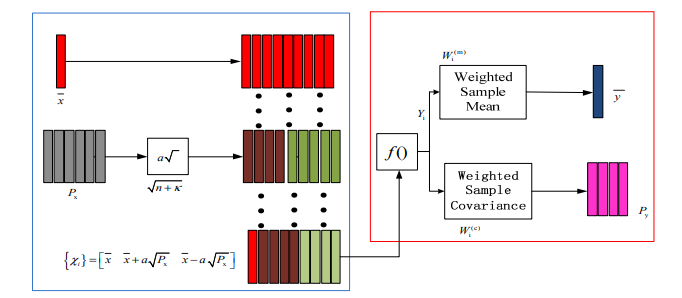
\includegraphics[width=0.8\textwidth]{Chap07/Figures/UKF_UT.PNG}
	\caption{UKF UT Transformation }
	\label{fig:UKF_UT_Transformation}
\end{figure}
Estimate using the Kalman filter standard: Since the state space for SoC estimation is the same as that for EKF, we can easily demonstrate the unscented Kalman filter technique as follows:


\textbf{Initialization:}\\
\begin{equation} \label{eq:UKF_initialization}
    \bar{x_0} = \textbf{E}(x_0) , P_0 = \textbf{E}[(x_0 - \bar{x_0})(x_0 - \bar{x_0})^{T}] \\
\end{equation}  
State Initialization refers to the equation \ref{eq:UKF_state_initialization}.

\textbf{Time Update:}\\
State estimate time update:  \\
\begin{equation} \label{eq:UKF_State_estimate_time_update}
    x_{k/k-1} = f(x_{k-1},x_{k-1}^{v}), \bar{x_{k/k-1}} = \sum_{i = 0}^{2n} W_i^{(m)}x_{i,k/k-1} \\
\end{equation}  

Error covariance time update: \\
\begin{equation} \label{eq:UKF_Error_covariance_time_update}
    P_{x,k/k-1} = \sum_{i = 0}^{2n} W_i^{(c)}[(x_{i,k/k-1} - \bar{x_{i,k/k-1}})(x_{i,k/k-1} - \bar{x_{i,k/k-1}})^{T}] \\
\end{equation}  

Output estimate time update: \\
\begin{equation} \label{eq:UKF_Output_estimate_time_update}
    Y_{k/k-1}  = g(x_{k/k-1},x_{k/k-1}^{n}),  \bar{y_{k/k-1}}  = \sum_{i = 0}^{2n_a} W_i^{(m)}Y_{i,k/k-1}\\
\end{equation}  

\textbf{Measurement is updated:} \\
Estimator gain matrix: \\
\begin{equation} \label{eq:UKF_Estimator gain matrix}
    \begin{split}
        P_{y,k} & =  \sum_{i = 0}^{2n} W_i^{(c)} (Y_{i,k/k-1}  - \bar{y})(Y_{i,k/k-1}   - \bar{y})^{T}  \\
        P_{xy,k} & =  \sum_{i = 0}^{2n} W_i^{(c)} (Y_{i,k/k-1}  - \bar{x})(Y_{i,k/k-1}   - \bar{y})^{T} \\
        \textbf{K} &= P_{xy,k} \times P_{y,k}^{-1}  \\
    \end{split}
\end{equation}  

State estimate update: \\
\begin{equation} \label{eq:UKF_State_estimate_update}
     \hat{x_k} = \hat{x_k^{-}} + K (y_k - \hat{y_k^{-}} )  \\
\end{equation}  

Error covariance measurement update:\\
\begin{equation} \label{eq:UKF_Error_covariance_measurement_update}
    P_{x,k} = P_{x,k}^{-}  -  K P_{y,k} K^{T} \\
\end{equation}  

The process can be expressed as shown in Figure \ref{fig:SoC_estimation_based_on_UKF}
\begin{figure}[h]
    \centering
    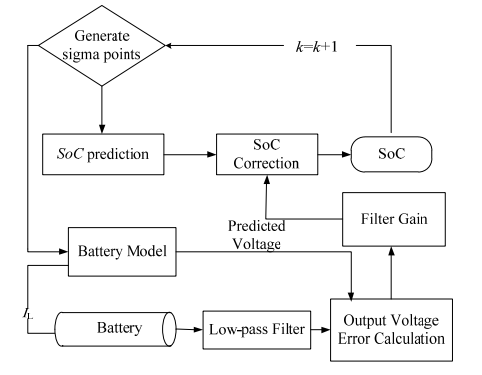
\includegraphics[width=0.5\textwidth]{Chap07/Figures/SoC_estimation_based_on_UKF.PNG}
    \caption{SoC estimation based on UKF }
    \label{fig:SoC_estimation_based_on_UKF}
\end{figure}

\subsection{Adaptive Unscented Kalman Filter}
To determine the battery's SOC, the extended Kalman filter (EKF) was developed. This approach views the SOC as a state variable and may estimate the dynamic system state using the least-squares method. The EKF, on the other hand, is forced to linearize the nonlinear system function using the Taylor series expansion, thus it ignores the high-order elements and invariably makes mistakes. Unscented transform (UT) is used by the unscented Kalman filter (UKF) to handle nonlinear issues. The estimate precision is increased compared to the EKF approach because it doesn't require computing the Jacobian matrix and doesn't overlook high-order terms \cite{Adaptive_UKF_for_SOC_Estimation}.
The particle filter (PF) employs a statistical approach that can be effective for nonlinear issues and does not need that the measurement noise and the observation noise follow a Gaussian distribution, however, this algorithm's computation is complicated.
The strong tracking unscented Kalman filter is used in literature, but to calculate the strong tracking factor, it is also necessary to compute the Jacobian matrix, which increases the computing work.

The UKF (and EKF) algorithm, the strong tracking filter, and the adaptive algorithm are all combined in the adaptive strong tracking unscented Kalman filter (ASTUKF) algorithm. Unlike other strong tracking filters, this method does not need to calculate the Jacobian matrix, which lessens the computational load. This approach can increase tracking and robustness to sudden changes and can fix the SOC estimating mistake brought on by model error [\cite{LIPO_AUKF_Meng},\cite{Comparision_EKF_UKF_He}].

The Adaptive Unscented Kalman Filter forced inherits all the implementation steps from UKF, AUKF takes the approach that the residual sequence remains orthogonal to one another by adding a fading component to the state-prediction covariance matrix and adjusting the gain matrix in real-time. The AUKF method has been refined by literature and no longer requires computing the Jacobian matrix. The battery model mistake can affect the battery's SOC estimation. We employ the AUKF approach as a SOC estimator because it can increase estimate accuracy and decrease SOC estimation error brought on by model imbalance.

The process of determining the fading factor $\gamma _{k+1}$ :\\

\begin{equation}\label{eq:AUKF_fadding_factor}
	V_{k+1}=\begin{cases}
	  e(1)e(1)^{T}, & \text{K=0}.\\
	  \frac{\rho V_k + e(k+1)e(k+1)^{T}}{1 + \rho}, & \text{$K \geq 1$}.\\
	\end{cases}
\end{equation}
Where, $e(k+1) = Y_{k+1} - \bar{Y_{k+1/k}}$, $\rho$ is forgetting factor, $ 0 \leq  \rho \leq 1 $ \\

\begin{equation}
	\begin{cases}
	  N_{k+1} & = V_{k+1} - \beta R_{k+1} \text{where R is Noise covaraince matrix}\\
      M_{K+1} & =  \sum_{i = 0}^{2n} W_i^{(c)} (Y_{i,k+1/k}  - \bar{Y_{k+1/k}})(Y_{i,k+1/k}   - \bar{Y_{k+1/k}  })^{T} \\
	\end{cases}
\end{equation}
\begin{equation}
    \gamma _{0} = \frac{tr N_{k+1} }{ tr M_{k+1}} \\
\end{equation}

\begin{equation}
    \gamma _{K+1}=\begin{cases}
                    \gamma _{0}   & \text{$\gamma _{0}$  > 1}\\
                    1   & \gamma _{0}  \leq 1 \\
    \end{cases}
\end{equation}

Then the state covariance matrix is updated: \\
\begin{equation}
    \begin{cases}
    P_{y_k,y_k}& = \gamma _{K+1} \sum_{i = 0}^{2n} W_i^{(c)} (Y_{i,k+1/k}  - \bar{Y_{k+1/k}})(Y_{i,k+1/k}   - \bar{Y_{k+1/k}  })^{T} + R_k \\
    P_{x_k,y_k}& = \gamma _{K+1} \sum_{i = 0}^{2n} W_i^{(c)} (X_{i,k+1/k}  - \bar{X_{k+1/k}})(Y_{i,k+1/k}   - \bar{Y_{k+1/k}  })^{T} + R_k \\
    P_{k+1/k+1}& = \gamma _{K+1} P_{k+1/k+1} - K_{k+1} P_{y_k,y_k} K_{k+1}^T .\\
    \end{cases}
\end{equation}


The AUKF approach adds a fading component to the state-prediction covariance matrix, which maintains good tracking performance, reduces error brought on by model uncertainty, and dynamically modifies the noise covariance matrix. As a result, the AUKF approach, which combines the benefits of the two algorithms EKF, UKF, and AUKF, can produce estimates with a better degree of accuracy.

In contrast to the conventional UKF, the AUKF untraced Kalman filter integrates the AUKF reasoning process to correct the system's measurement noise on the fly. The covariance of the measurement noise is adjusted using the difference between the theoretical value and the actual value of the measured noise along with AUKF reasoning, and the corrected covariance is then added to the output equation to update the system.

\section{Comparision of Kalman Algorithms Results}
The results from Kalman sub-algorithms are quite elegant, I have made distinguished all the algorithms are Kalman algorithms by their soc estimation and error deviation from the true soc of the battery \ref{fig:Kalman_Algorithms_Battery_Charing_SOC_Comparision}.
I also took an opportunity to summarize \ref{fig:Kalman_Algorithms_Battery_Charing_SOC_Comparision}(b) the error deviation from the true soc to the estimated soc, it is very clear from the results that Columb soc estimation performing very poorly compared to all remaining algorithms. Each Kalman algorithm from the extended Kalman algorithm to the adaptive Kalman algorithm one performs better than the others. Deciding which is best is very much self-explanatory from the distinguished results \ref{fig:Kalman_Algorithms_Battery_Charing_SOC_Comparision}. Thanks to the battery model that is presented in  
chapter \ref{ch:Battery_Modeling_Emulation}, is the fundamental foundation for all the algorithms that we have seen all over. Then there is an obvious question why don't we choose the best algorithm among all, well we can but the problem is if we go for the higher-end algorithms the computational power increases exponentially. And it becomes and bottom neck for the small-scale embedded application. The algorithm once can choose based on the measurement setup, computational power, application use case, and many other factors.
\begin{figure}[h]
	\centering
	\subfigure[Kalman Algorithms Battery Charing SOC Estimation ]{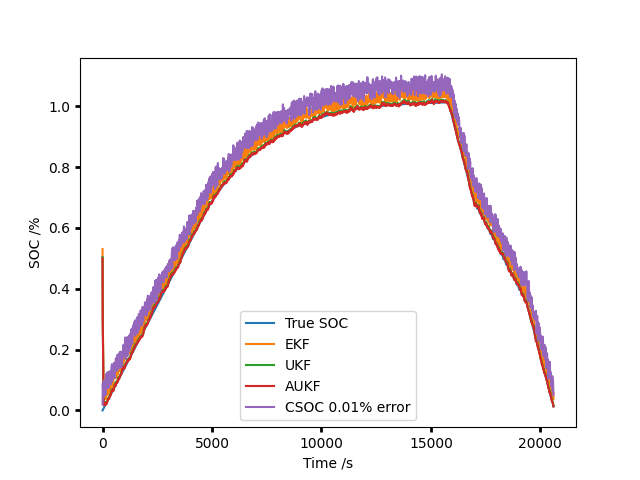
\includegraphics[scale=.4]{Chap07/pyKalmanFilter/Python/Figures/BatteryChargingSOC_Comparriosn.png}}
	\qquad
	\subfigure[Kalman Algorithms Battery Charing SOC Estimation Error Comparision]{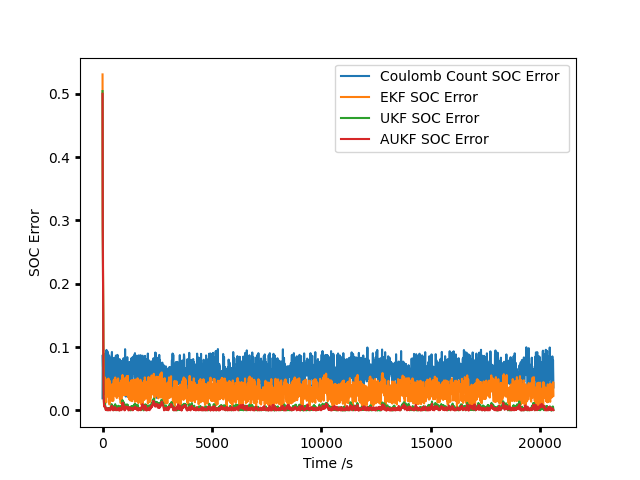
\includegraphics[scale=.4]{Chap07/pyKalmanFilter/Python/Figures/BatteryChargingSOCError_Comparrison.png}}
	\caption{Kalman Algorithms Battery Charing SOC Comparision}
	\label{fig:Kalman_Algorithms_Battery_Charing_SOC_Comparision}
\end{figure}

\subsubsection{Convergence of Kalman Algorithms :}
I have summarized the convergence of the algorithms in figure \ref{fig:Kalman_Algorithms_Convergence}, extended Kalman filter is converging slower compare to the adaptive Kalman filter algorithms, let me take a moment to explain what causes them for convergence. In the extended Kalman filter picking the initial condition is very much simple and the convergence matrix is very much diversified from the measuring results in the setup which is why it takes more iterations to get converge. UKF takes a random process approach it selects the mean from the measuring data as the initial state and the variance of the measuring data as the covariance matrix. The AUKF forced the residual sequence to remain orthogonal to each other by adding a fading factor to the state-prediction covariance matrix and adjusting the gain matrix in real-time. The AUKF method has been refined by literature and no longer requires computing the Jacobian matrix. The battery model mistake can affect the battery's SOC estimation. We employ the AUKF approach as a SOC estimator because it can increase estimate accuracy and decrease SOC estimation error brought on by model imbalance.

\begin{figure}[h]
	\centering
	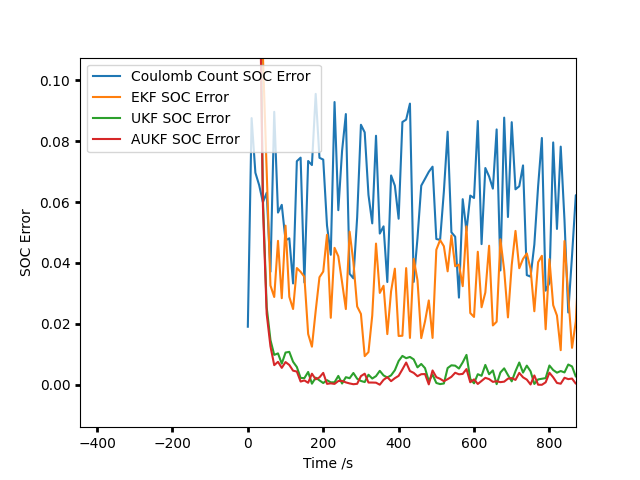
\includegraphics[width=0.6\textwidth]{Chap07/pyKalmanFilter/Python/Figures/KalmanAlgorithms_convergence.png}
	\caption{Kalman Algorithms Convergence }
	\label{fig:Kalman_Algorithms_Convergence}
\end{figure}



\section{Summer of the Chapter \ref{ch:Battery_SOC_Estimation_Algorithms}}
All over in chapter \ref{ch:Battery_SOC_Estimation_Algorithms}, I took an effort to gather focus on the Kalman approach to estimating the soc, is it only the algorithm in the literature well certainly not there are plenty of approaches are there in the literature to estimate the soc of the battery. Then a very obvious question is why Kalman's approach? Well, the answer is it is very immune to noise and accurate estimation, and it has proven most algorithms over decades. As an extension of this topic, we can use much more advanced approaches with Kalman, for instance, fuzzy networks with Kalman filter, support vector machines with Kalman, and many others... I have limited this chapter to 3 or 4 (Amper second, Kalman, EKF, UKF, AUKF) types of algorithms for soc estimation. Even we can look into machine learning, AI, and neural network approaches like the random forest, gradient descent, and stochastic gradient descent, etc. machine learning algorithms are more elegant and robust, but the drawback with those algorithms is we need a large amount of data to characterize the algorithms and tune, perhaps millions of data.  So it is not so easy to go ahead with the machine learning approach in smaller firms. Well, then Kalman's approach is the best among all? Not really it has drawbacks as well, but it holds sufficient grounds for estimating the battery soc.